Ce projet consiste à créer un outil auteur de mini-jeux 3D destinés au Web.
En effet, les récentes arrivées de HTML 5 et d'outils 3D comme WebGL permettent désormais l'affichage d'objets 3D directement
intégrés dans les pages internet.
Cependant, les contenus 3D dans les pages Web ne sont actuellement que très peu interactifs.
Fort du succès des jeux flash, les contenus interactifs 3D comme les mini-jeux ont naturellement leur place sur le Web.
Or s'il existe de nombreux outils tel que Google SketchUp pour créer et manipuler les objets 3D en eux-mêmes.
Il reste tout de même un effort important à faire en ce qui concerne les interactions avec ceux-ci et en particulier la création de mini-jeux en 3D.

\begin{figure}[h]
 \centering
 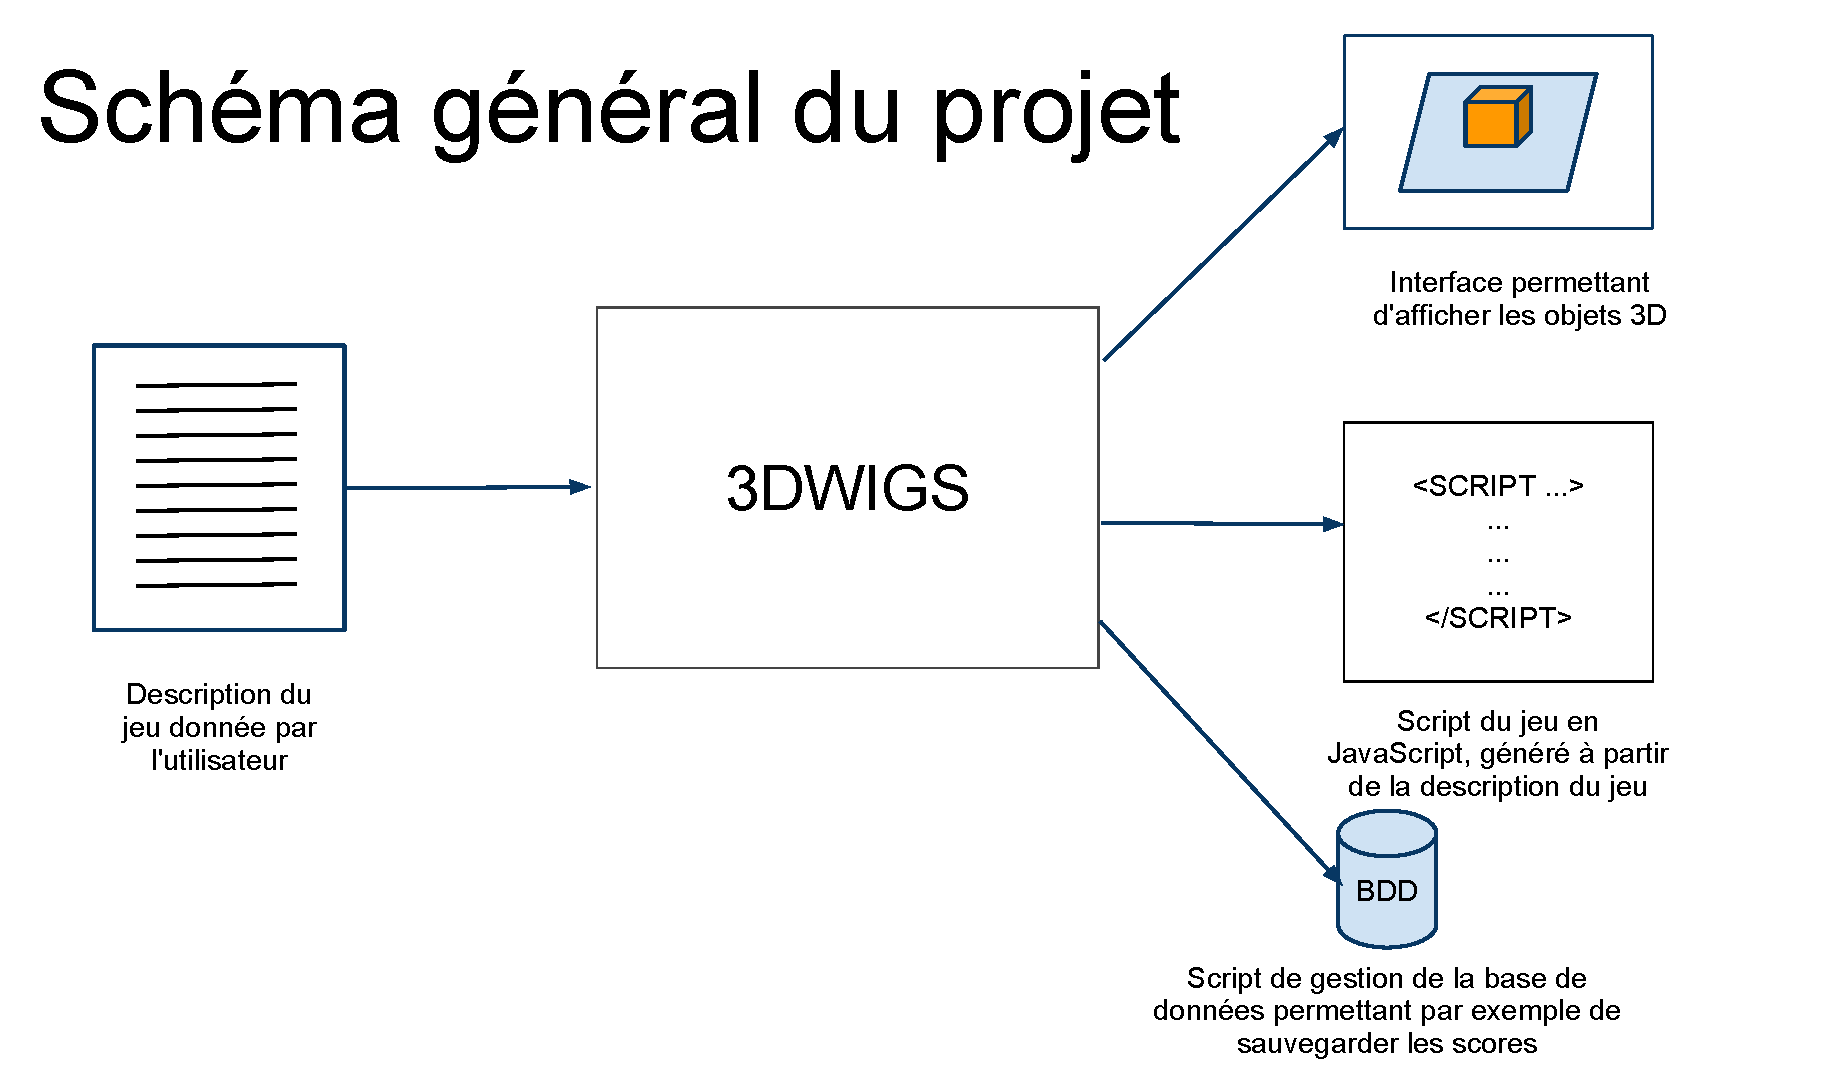
\includegraphics[height=7.5cm]{img/schema_general}
\end{figure}

La conception d'un outil de création de mini-jeux 3D pour le Web nécessite, d'une part la description des objectifs, des règles, des interactions, 
du scénario du jeu qui permettra de générer le code du jeu, et d'autre part les éléments 3D constitutifs.
Il peut également être souhaitable de pouvoir sauvegarder une partie :
un jeu ne se finit pas nécessairement en quelques minutes, le fait de pouvoir reprendre une partie commencée un autre jour est alors nécessaire.

\vspace{0.2cm}

La figure ci-dessus présente le principe général de l'outil.
La partie gauche représente un fichier écrit par l'utilisateur contenant les règles du jeu qu'il souhaite créer respectant
une certaine syntaxe qu'il faut définir.

Il s'agit de créer un langage, à la fois suffisamment abstrait pour être accessible à n'importe quel utilisateur, mais également suffisamment riche
pour pouvoir décrire un maximum de jeux.
Le langage est défini par une grammaire.
Cette dernière doit permettre de décrire à la fois :
\begin{itemize}
 \item les objectifs ;
 \item les règles ;
 \item les interactions avec le(s) joueur(s).
\end{itemize}

La création de la grammaire est complexe. En effet, il existe de nombreuses catégories de jeux.
Par exemple, un jeu de gestion n'a, à première vue, aucun point commun avec un jeu de volley ou un jeu de plateforme.

Il serait illusoire de vouloir décrire tous les jeux à l'aide d'une seule et unique grammaire, à cause de leurs différences.
Toutefois, de nombreuses similarités existent entre plusieurs jeux. Il s'agit donc de les exploiter afin de définir un langage général de description de jeux.

Le fichier définissant le jeu via la grammaire se fera à l'aide d'un éditeur spécial, créé à l'aide d'Eclipse par exemple.

La partie centrale du schéma correspond à un compilateur.
Il permet de convertir le fichier de description du jeu en code JavaScript exécutable dans une page Web.
En effet, le langage JavaScript a été choisi pour la génération du jeu car toutes les interactions se font côté client.

La création et l'édition des objets 3D se fera à l'aide d'outils déjà très complets tel que Google SketchUp.
Leur affichage sera géré par WebGL, une spécification d'affichage 3D pour les navigateurs. 
Elle permet d'utiliser le standard OpenGL depuis le code JavaScript d'une page web, 
exploitant les accélérations matérielles 3D à l'aide des pilotes OpenGL de la carte graphique